%%%% Proceedings format for most of ACM conferences (with the exceptions listed below) and all ICPS volumes.
\documentclass[sigconf]{acmart}
\usepackage{paralist}
\usepackage{url}
\usepackage[hyphenbreaks]{breakurl}

\def\UrlBreaks{\do\/\do-}

%%%% As of March 2017, [siggraph] is no longer used. Please use sigconf (above) for SIGGRAPH conferences.

%%%% Proceedings format for SIGPLAN conferences 
% \documentclass[sigplan, anonymous, review]{acmart}

%%%% Proceedings format for SIGCHI conferences
% \documentclass[sigchi, review]{acmart}

%%%% To use the SIGCHI extended abstract template, please visit
% https://www.overleaf.com/read/zzzfqvkmrfzn

\usepackage{booktabs} % For formal tables


% Copyright
%\setcopyright{none}
%\setcopyright{acmcopyright}
\setcopyright{acmlicensed}
%\setcopyright{rightsretained}
%\setcopyright{usgov}
%\setcopyright{usgovmixed}
%\setcopyright{cagov}
%\setcopyright{cagovmixed}

\copyrightyear{2018}
\acmYear{2018}
\setcopyright{acmlicensed}
\acmConference[Koli Calling '18]{18th Koli Calling International Conference on Computing Education Research}{Koli, Finland}
% ACM had "Computing" instead of Computer, please update
%\acmBooktitle{}
%\acmPrice{15.00}
%\acmDOI{10.1145/3159450.3159547}
%\acmISBN{978-1-4503-5103-4/18/02}
% This slight change to the code may also save 1 or 2 lines of space.

% removes the headers from each page per the preparation instructions, as these are not needed and will be updated with the chairs' actual session names during the pagination/indexing process:
\fancyhead{}

\begin{document}
\title{Ioc TBC}
%\titlenote{}
%\subtitle{Extended Abstract}
%\subtitlenote{}

\author{James H. Davenport}
\affiliation{%
  \institution{University of Bath}
  \streetaddress{}
  \city{Bath} 
  \country{United Kingdom}
}
\email{j.h.davenport@bath.ac.uk}

\author{Rachid Hourizi}
\affiliation{%
  \institution{University of Bath}
  \streetaddress{}
  \city{Bath} 
  \country{United Kingdom}
}
\email{r.hourizi@bath.ac.uk}

\author{Tom Crick}
\affiliation{%
  \institution{Swansea University}
  \streetaddress{}
  \city{Swansea} 
  \country{United Kingdom}
}
\email{thomas.crick@swansea.ac.uk}

 
% The default list of authors is too long for headers}
%\renewcommand{\shortauthors}{Davenport, Hourizi and Crick}


\begin{abstract}
% abstract to do at the end
\end{abstract}

\keywords{TBC}

\maketitle

% From CfP:
% Short papers (up to 5 pages) focus on dissemination and discussion
% of new ideas in computing education practice or research that merit
% wider awareness and discussion within the community. They can present
% preliminary results of new educational innovations, present and
% discuss novel educational technologies, report work-in-progress
% research (including promising systems or tools that have not yet been
% evaluated and/or adopted extensively), or raise issues of significance
% for the development of the discipline, such as long-term strategic
% needs for computing education and curricula. All short papers are
% expected to have an appropriate coverage of literature to support the
% ideas and arguments that they present. Because it lacks some elements
% of a research paper, a short paper is evaluated mainly by its
% anticipated impact on discussions during the conference and possible
% future contribution to the field of computing education.

% TC: need more UK context here, I can add this -- do we want to have
% this framed as a paper to justify/introduce the IoC, as well as
% other UK interventions? Framed as a discussion piece with
% transferability elsewhere?

\section{Introduction}
Superficially, the employment outlook for computing graduates in the UK looks excellent. \cite[p.~74]{UKCES2015b} states
\begin{quote}
the digital sub-sector will need 518,000 workers for roles in the three highest skilled occupational groups. However, over the last ten years only 164,000 individuals graduated from a first degree in computer science.
\end{quote}
This is profitable for the individual: according to \cite[Figure 4]{BIS2011a}, ``mathematical and computer sciences'' have the second highest earnings return of all subjects (beaten only by ``medicine and dentistry'').
The country profits from this as well: according to
\cite[p.~16]{BIS2011a}, this is, per head, the fourth most beneficial
subject to the Exchequer.

\section{So What's the problem}
Despite the headline success in \cite{BIS2011a}, the employment
figures are not great, and the earnings data are patchy.

\subsection{Employment}
Quoting \cite{UKCES2015b}, the author of a UK Government-commissioned report \cite{Shadbolt2016a} writes
\begin{quote}
In this context, apparently high rates of unemployment\footnote{11.7\% six months after graduation (the standard UK measure) at the time of \cite{Shadbolt2016a}, compared with a STEM average of 8.4\%. Note, however, that Computing is 20\% of STEM \cite[Table 1]{Wakeham2016a}, so `STEM-less-Computing' has a 7.6\% unemployment rate.} amongst graduates of Computer Sciences and other STEM\footnote{STEM is ``Science, Technology, Engineering, Mathematics'' for \cite{Shadbolt2016a} and this paper.} courses demanded an explanation. 
\end{quote}
A significant explanation is ``There are notable differences in the characteristics of Computer Sciences entrants compared to entrants in other STEM subjects'' \cite[\P2.6]{Shadbolt2016a}: fewer women, but
\begin{description}
\item[50\% more] mature students,
\item[16\% more]Black and Minority Ethnic (BME) and 
\item[40\% more]students from backgrounds where people have traditionally not participated in HE (LPNs).
\end{description}
Mature, BME and LPN students all find getting jobs more difficult.
\par
However, for those students that do find jobs, the data are better,
showing \cite[Figure 6]{Shadbolt2016a} fewer students in
``non-graduate jobs'' or low-earning jobs than in STEM as a whole.

\subsection{Earnings}
If we look beyond purely getting jobs to the earnings\footnote{Clearly not the only measure of job quality, or contribution to society, but at least it's measurable, and has been measured in the LEO dataset \cite{DfE2017a}, which tracks individuals through school, university and into the labour market, combining educational, tax and benefits data.}, the position (as described in \cite{DfE2018d}, and presented to the public in \cite{BBC2018f}, which also allows the reader to break down the data by university and subject.) is even less clear on a microscopic level, though on a macroscopic level it bears out much of what \cite{Shadbolt2016a} said.

On the macroscopic level, the reader should consider \cite[Table 5]{DfE2018d}. We focus on the `Men' data as presented here, as there are (regrettably) many more than there are women in the cohorts, though the effects are similar. This shows that an OLS (``Ordinary Least Squares'') fit shown that a man reading Computing would earn 3.3\% more than had he read a subject at random. If one corrects for prior attainment, this rises to 10.5\%, and 12.6\% if other factors are taken into account. For reasons explained in \cite[\S4.2]{DfE2018d}, the authors prefer IPRWA (``Inverse Probability Weighted Regression Adjustment''), and this moves the earning difference to 14.7\%. For men, the overall effect of these adjustments is to move Computing from being middle-of-the-pack \cite[Figure 15]{DfE2018d} to fourth best  \cite[Figure 17]{DfE2018d}, and for women is moves to seventh best  \cite[Figure 16]{DfE2018d}.

\subsection{Per-University Earnings}
\cite{BBC2018f} allows one to break down the data underpinning \cite{DfE2018d}, and the Computing figures are challenging.  
Salary premiums, allowing for the factors described above, are reported separately for men and women, and only if there were at least 50 students of that gender in the five cohorts (graduation 2007--8 to graduation 2011-12) considered. This means that, of the 82 English universities reporting computing, 80 report male data and 30 report female data --- 28 report both. Looking at the 28 (see Figure \ref{fig:BBC}), one's first impression is that the male and female data are uncorrelated: for example the two universities with male premiums just above +\pounds2500 have female premiums of +\pounds9325 and -\pounds5793. There is in fact a definote ($p=0.0034$) positive correlation, but a fairly weak one ($R^2=0.286$). 
\begin{figure}\caption{\label{fig:BBC}}
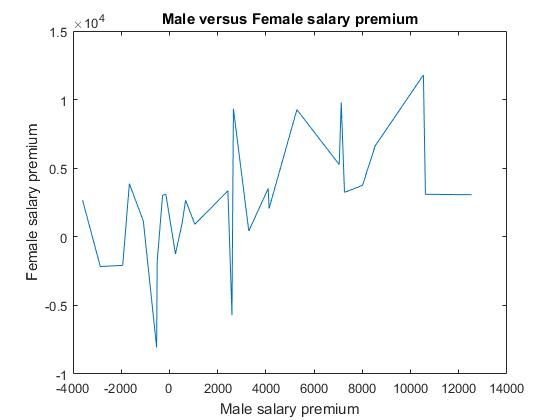
\includegraphics[scale=0.45]{BBCSalaryData.jpg}
\end{figure}
%Overall framing for the paper, etc

\section{UK Policy Context}
It is worth recalling that, after the Government's acceptance of the Browne report \cite{BIS2010a}, students in England pay probably the highest\footnote{Or possibly second-highest after US students, but the US averages in \cite[Table B5.1]{OECD2016a} conceal an enormous variation.} prices in the world for undergraduate education: between \pounds6000 and \pounds9000/year for tuition alone. While this is normally covered by student loans repaid on an income-contingent basis, essentially through a 9\% income tax premium, there is evidence \cite{CallenderMason2017a} that this ``contribute[s] to lower rates of planned H[igher] E[ducation] participation by lower-class students''.

The Government has also launched ``Degree Apprenticeships'' \cite{BIS2015a}. These were described by the then Prime Minister as ``combining a full degree with the real practical skills gained in work and the financial security of a regular pay packet''. The employer pays the tuition cost, but due to the Apprenticeship Levy \cite{HMRC2016a}, most employers will find there is no net cost.

Set the scene -- UK digital skills, CS ed reform, digital economy, etc

Cite previous work on programming~\cite{davenport-et-al:latice2016,murphy-et-al:programming2017,simon-et-al:sigcse2018}

Cite previous policy-related work~\cite{crick+sentance:2011,brown-et-al-sigcse2013,brown-et-al-toce2014,crick+moller-wipsce2015}

\section{Skills mismatch}
There is a widespread and longstanding complaint that ``students aren't industry-ready'', or ``there is a skills mismatch''. Some of this is due to a misapprehension on the part of employers (generally those outside the IT industry itself, but seeking to hire people wih ``10 years experience of programming in Ruby''), but much of it is genuine. One of the main challenges for the university community is to understand this complaint.

\subsection{Sandwich Years}
In the U.K. context, a university course that includes a period working in industry (which may include government, charity etc.) is generally called ``sandwich'', and in North America the term ``co-op'' is generally used. The most common model in Computing in England, where the vast majority of students study three-year Bachelor's degrees, is a year's placement in industry between the second and final years of study. This is remarkably successful in computing. The University of Bath has run such courses since its founding (1966), with about 80\% of students opting to take the sandwich year. There is statistical evidence for its success wherever it is used in the U.K.\footnote{And at least anecdotal evidence elsewhere: ``the co-op system is a major reason for our [University of Waterloo] success'' \cite{Watt2017a}.}:
\begin{quote}
those studying sandwich courses enjoy the lowest levels of unemployment (6\% sandwich vs 15\% non-sandwich), the lowest levels of non-graduate level employment (6\% sandwich vs 25\% non-sandwich), and graduates from sandwich courses are twice as likely to be earning over \pounds20,000 compared to those who did a standard degree. \cite[\P2.5]{Shadbolt2016a}
\end{quote}
A simplistic remedy would be to require that all students study sandwich degrees, but this has numerous objections:
\begin{enumerate}
\item Some students do not wish to, often for valid reasons;
\item The supply of employers willing to offer such placements is limited, and often they are only offered to a limited nmber of universities with whom the employer has built up relations, often going back decades;
\item The university needs to invest in the process: a sandwich year is not a matter of simply allowing studnts to intermit their studies.
\end{enumerate}
Hence we should ask ourselves \emph{why} such courses are so successful.  There are, it seems to the authors, two classes of reasons: those instrinsic to the sandwich process, and the skills the sandwich process confers. The first class is easy to understand: the employer can view the year as a year-long assessment phase before deciding whether to offer a permanent job. Bath's experience is that about 2/3 of sandwich placements result in job offers to the student. However, it is the second class that we need to investigate. A major one, brought out repeatedly by students returning from placement, is team working.
\subsection{Team/Group working}
``Teamwork'' is often identified as a key skill \cite[and many others]{ArcherDavidson2008}. Simplistically, then, universities should teach it. Indeed, the British Computer Society has long required this of degrees it accredits:
\begin{quote}
An ability to work as a member of a development team recognising the different roles within a team and different ways of organising teams \cite[Requirement 2.3.1]{BCS2018a}.
\end{quote}
\section{Institute of Coding}
Formally announced in \cite{DfE2018a}, but foreshadowed in \cite{HMG2015a}.
% From CfP:
% Short papers (up to 5 pages) focus on dissemination and discussion
% of new ideas in computing education practice or research that merit
% wider awareness and discussion within the community. They can present
% preliminary results of new educational innovations...

% TC: so are we going to talk about the IoC "national" model, with
% industry matched funding, etc?

\section{Anticipated Impact}

\section{Conclusions and Future Work}

% TC: what is the main takehome from this paper? Replicability to
% other jurisdictions? Introducing the IoC as an effective
% educational/industrial collaboerative intervention? Recognising all
% of the mistakes/missed opportunitirs from before, even though
% significant government policy in this space, etc? Global
% competitiveness, etc
% also: directly linking to CAS/BCS work, curriculum+quals reform, pipelines, perceptions?

\section{Acknowledgements}
This work was supported by the Institute of Coding which received
\pounds20m of funding from the Office for Students, and support from
the Higher Education Funding Council for Wales (HEFCW).  The first
author is grateful to Matt Dickson (Bath) for discussions about
\cite{DfE2018d}, but any mistakes are the authors' alone.


\bibliographystyle{ACM-Reference-Format}
\bibliography{kolicalling2018} 

\end{document}
